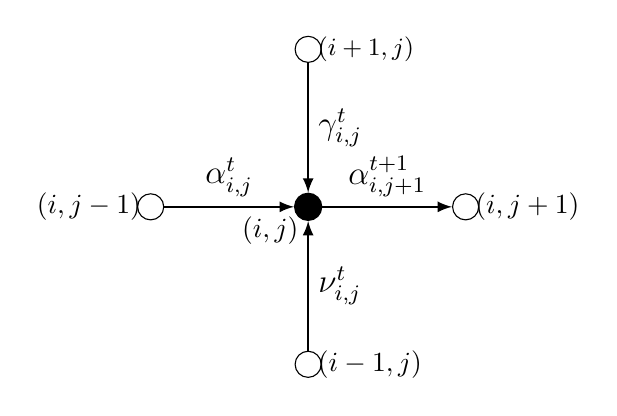
\begin{tikzpicture}[>=latex,
point/.style={circle,radius=\r,draw,thick,fill=black},
neighbor/.style={circle,radius=\r,draw}]
\def\r{0.2}
\node[point] (C) at (0,0){};
\node[neighbor] (N) at (0,2){};
\node[neighbor] (S) at (0,-2){};
\node[neighbor] (E) at (2,0) {};
\node[neighbor] (W) at (-2,0){};

\node[right] at (N) {\small{$(i+1,j)$}};
\node[right] at (S) {$(i-1,j)$};
\node[left] at (W) {$(i,j-1)$};
\node[right] at (E) {$(i,j+1)$};
\node [below left] at (C) {$(i,j)$};

\draw [thick,->] (C) to node[above]{\large{$\alpha_{i,j+1}^{t+1}$}} (E);
\draw [thick,->] (W) to node[above]{\large{$\alpha_{i,j}^{t}$}} (C);
\draw [thick,->] (N) to  node[right]{\large{$\gamma_{i,j}^{t}$}} (C);
\draw [thick,->] (S) to node[right]{\large{$\nu_{i,j}^{t}$}} (C);

\end{tikzpicture}
